\documentclass[examenvragen.tex]{subfiles}

\begin{document}

\section{Verschillende basis}

\subsection{Opgave}
Gegeven de volgende definitie van $e$ willen we $e$ benaderen.
\[
\lim_{x\rightarrow\infty}\left(1+\frac{1}{x}\right)^x = e
\]
We zullen $e$ benaderen op twee manieren door een iteratieproces waarbij de $k$-de benadering er als volgt uit ziet.
\[
e_{k} = \left(1+\frac{1}{x_k}\right)^{x_k}
\]
\begin{enumerate}
\item met $x_{k} = 2^k$
\item met $x_{k} = 10^k$
\end{enumerate}
We plotten de relatieve fout $\left| \frac{e_k - e}{e} \right|$ in functie van $k$ in figuur \ref{fig:vraag_verschillende_basis:rel_err}
We bekomen volgende grafieken voor de relatieve fout.
\begin{figure}[H]
\begin{center}
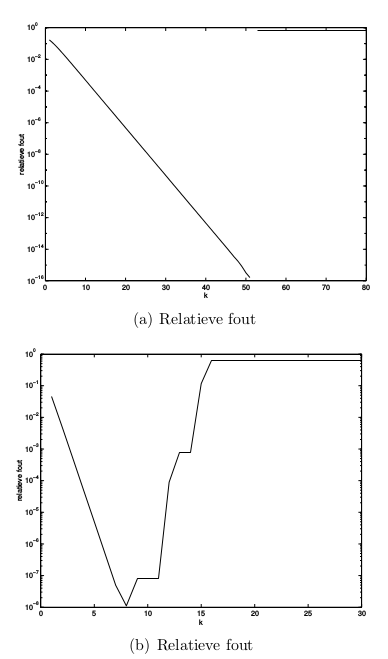
\includegraphics[scale=0.5]{illustraties/vraag_verschillende_basis.png}
\end{center}
\caption{Relatieve fout}
\label{fig:vraag_verschillende_basis:rel_err}
\end{figure}

\begin{enumerate}
\item Waarom zijn de twee grafieken zo verschillend?
\item Kan men hieruit afleiden met welke basis en met hoeveel beduidende cijfers de computer werkt?
\item Verklaar in detail je antwoord
\end{enumerate}

\subsection{Antwoord}
\subsubsection{Resultaten}
In de eerste grafiek zien we dat de relatieve fout afneemt tot $k$ groter wordt dan $52$. We zien bovendien dat de relatieve fout niet kleiner wordt dan $10^{-16}$. Daarna wordt de relatieve fout plot van grootteorde $10^{0}$.

In de tweede grafiek zien we dat de relatieve fout (enigszins sneller) afneemt tot $k$ groter wordt dan $7$, daarna wordt de fout weer groter tot ze ook van grootteorde $10^{0}$ wordt.

\subsubsection{Verklaring}
De benadering $e_k$ van $e$ wordt in het begin steeds beter omdat de theoretische formule (met de limiet) geldt. Op een bepaald punt worden de afrondingsfouten op $x_k$ echter groter dan de benadering beter wordt. De relatieve fout zal dan opnieuw stijgen.

Vanaf een bepaalde groote van $x_k$ wordt $\frac{1}{x_k}$ zo klein dat $1 + \frac{1}{x_k}$ geeft. $e_k$ wordt dan ook $1$ waardoor de absolute fout $e - 1$ wordt en de relatieve fout bijgevolg van grootteorde $10^{0}$.

\subsubsection{Antwoord op de vraag}
Op de verschillende $x_k$ worden verschillende fouten gemaakt. Bij de eerste worden er zelfs bijna geen fouten gemaakt op het berekenen van de $x_k$.

De computer werkt met basis $2$ omdat $2^k$ nagenoeg geen afrondingsfouten geeft. De computer werkt met ongeveer $16$ beduidende cijfers, of met $52$ bits in de mantisse.

\end{document}
